\section{Testing eBPF programs}\label{sec:testing}

We have built an elaborated testing infrastructure to test the P4 to C
compilers.  The infrastructure can perform both functional correctness
testing at the user level, and complete end-to-end testing by running
in the kernel.

\subsection{User-Space Testing}

User-space testing validates the correctness of the code generated by
compiler and can be performed even on systems that lack eBPF support
in the kernel.  The user space testing framework does not depend on
the LLVM~\cite{llvm} or any particular kernel version.  It also does
not require usage of \texttt{iproute2}~\cite{iproute} tooling such as
\texttt{tc} or \texttt{ip}.  It is also easier to debug failing tests
in user-space, by using tools such as GDB~\cite{gdb},
Valgrind~\cite{valgrind}, or Wireshark~\cite{wireshark}.

\begin{table}[h]
  \footnotesize
  \begin{center}
    \begin{tabular}{|p{3cm}|p{4.5cm}|} \hline
      \textbf{Command} & \textbf{Description} \\ \hline \hline
      \textbf{packet} port data & Insert a frame of bytes
      \textit{data} into port \textit{port}.    \\ \hline
      \textbf{expect} port data & Expect a frame of bytes
      \textit{data} on port \textit{port}.  \\ \hline
      \textbf{add} tbl priority match action & Insert a
      match-action entry with key \textit{match} and action
      \textit{action} into table \textit{tbl}. \\ \hline
      \textbf{setdefault} tbl action & Set the default action for table
      \textit{tbl}. \\
      \hline
      \textbf{check\_counter} tbl key==n & Check if the value on
      the entry \textit{key} in counter table \textit{tbl} matches
      \textit{n}.  \\
      \hline
      \textbf{wait} & Pause for a second. \\ \hline
    \end{tabular}
    \caption{The STF command palette.}\label{table:stf}
  \end{center}
\end{table}

\subsection{The Simple Test Framework}
\begin{figure}
  \centering
  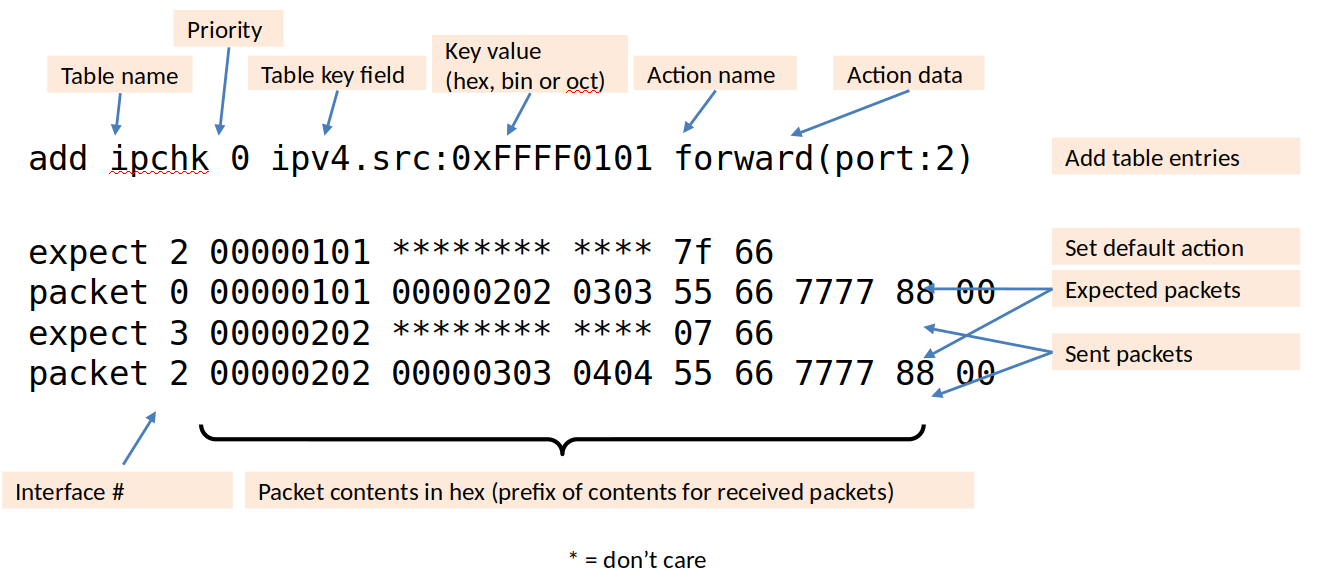
\includegraphics[width=\linewidth]{stf}
  \caption{Annotated example of a basic STF file.}
  \label{fig:stf}
\end{figure}

The P4 compiler includes a simple language (STF = Simple Testing
Framework) to describe input/output packets and to populate P4 tables.
Initially STF was used with software simulators to validate P4
programs, but we have adapted it for testing the eBPF and XDP
back-ends.  The STF framework is written in Python.
Figure~\ref{fig:stf} shows a small program written in the STF
language.  Table \ref{table:stf} describes the list of currently
supported STF operations in the eBPF testing backend.

The STF \texttt{packet} statement describes an input port and the
contents of a inbound packet.  The \texttt{expect} statement describes
an output port and the contents of an outbound packet.

Tables can be populated using the \texttt{add} statement, which
indicates a P4 table and an action to insert in the table, including
values for the action parameters.  Currently we assume that all
\texttt{add} statements are executed prior to all the packet
manipulation statements.

Our testing framework converts \texttt{packet} statements into Pcap
files, one for each input port tested.  \texttt{add} statements are
converted into C programs that populate eBPF maps.

Although STF supports testing counters as well, our eBPF testing
framework does not yet support this feature.

\begin{figure*}
	\centering
	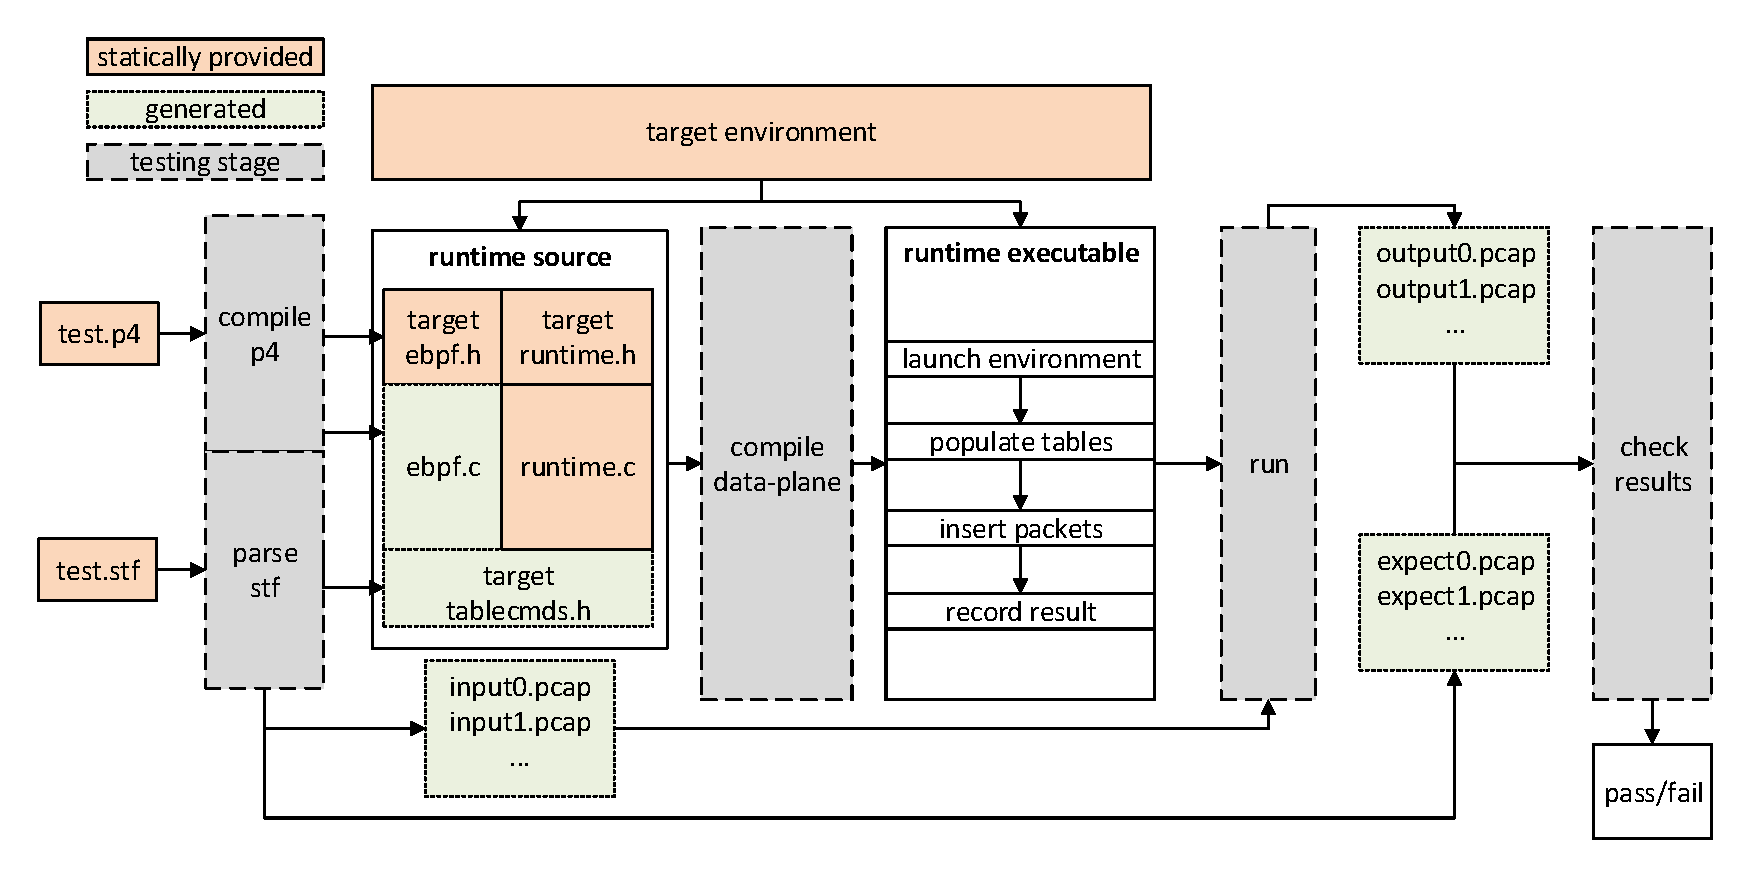
\includegraphics[width=\linewidth]{testing_workflow}
	\caption{Testing workflow for a P4-eBPF program. Environment and
		target are provided by the user.}
	\label{fig:p4_testflow}
\end{figure*}

\subsection{The Test Runtime}

Executing a P4 eBPF test is done in five stages (Figure
\ref{fig:p4_testflow}):

\begin{enumerate}
\item\textbf{compile-p4:} Compile the P4 file to C program.  This
  validates the P4 compiler.
\item \textbf{parse-stf:} Convert the STF file to a C program and into
  input PCAP files.
\item \textbf{compile-data-plane:} Compile and load the C programs
  into an executable.
\item \textbf{run:} Wire up the executable to read from the input PCAP
  files; run the executable -- first populate tables then execute the
  program over the input packets.  Capture the produced output packets
  into output files.
\item \textbf{check-results:} Compare the output packets with the
  expected results.
\end{enumerate}

\noindent These five stages look slightly differently when testing in
user-space and in kernel-space.

In user space we use a hash-table library to emulate eBPF maps.

When testing in kernel-space we compile the eBPF/XDP programs to eBPF
object files using LLVM.  Before the eBPF/XDP program is loaded, the
framework creates a bridge running in a network namespace.
Namespace-based isolation allows us to run multiple tests in parallel.
Virtual interfaces are attached to the bridge.  The testing runtim
injects packets into the associated ports using raw sockets. The
output results are recorded by attaching Tcpdump~\cite{tcpdump} to
each output virtual interface.
